\section{Resultados}
	Para comprobar la funcionalidad del programa, se realizó la siguiente prueba, se ingresó la cadena ``11''.\\
	Los resultados obtenidos fueron los siguientes:
	\begin{figure}[H]
		\begin{center}
			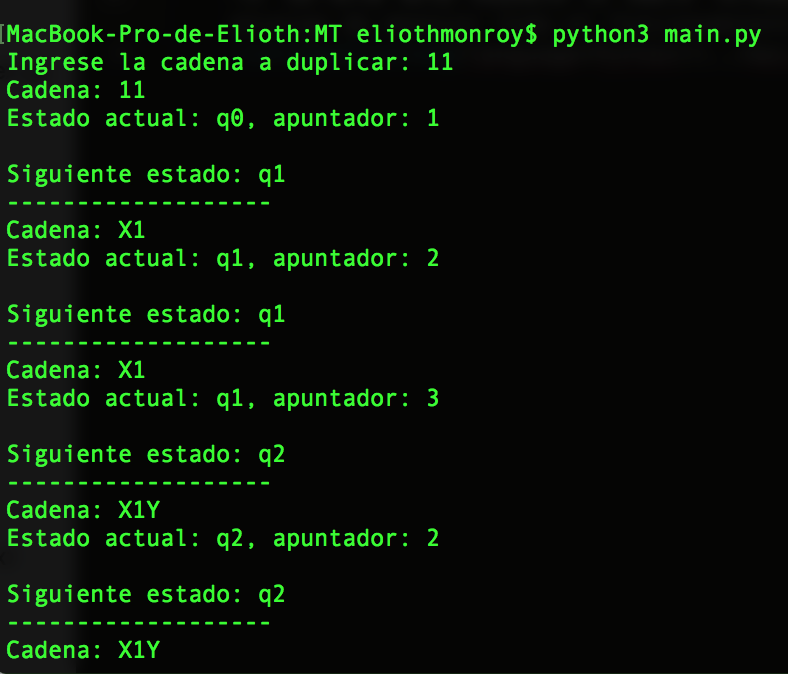
\includegraphics[scale=.6]{img/prueba1.png}
			\caption{Resultados prueba (1)}
			\label{fig:maquin2}
		\end{center}
	\end{figure}
	\begin{figure}[H]
		\begin{center}
			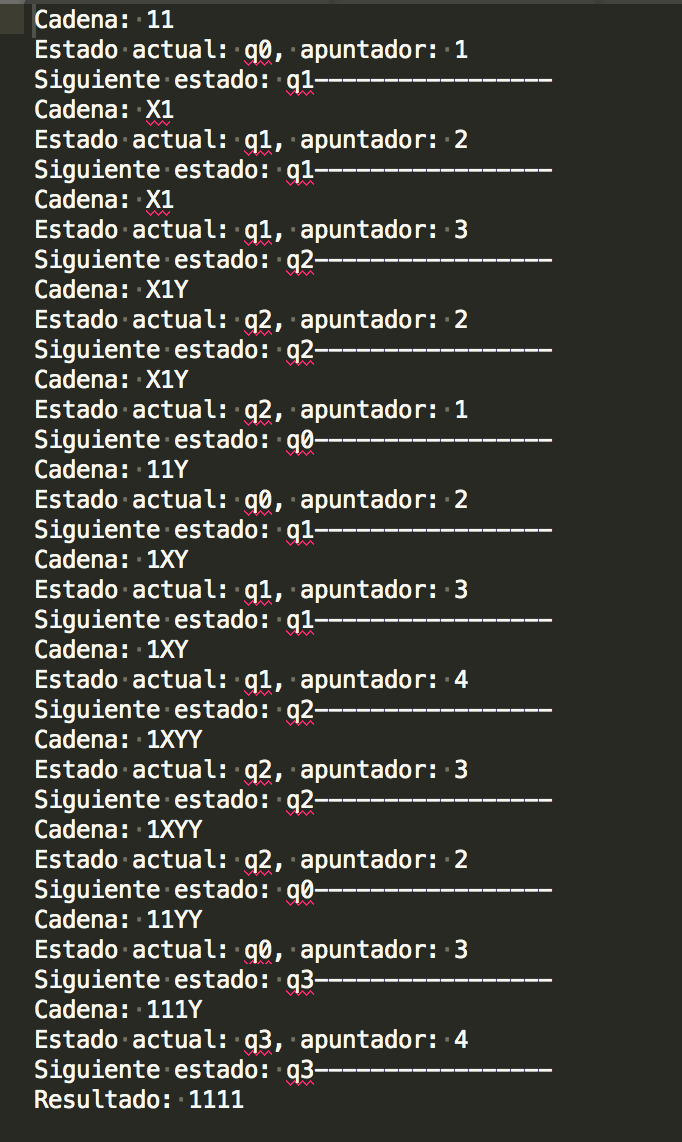
\includegraphics[scale=.6]{img/prueba2.png}
			\caption{Resultados prueba (2)}
			\label{fig:maquin3}
		\end{center}
	\end{figure}
	\begin{figure}[H]
		\begin{center}
			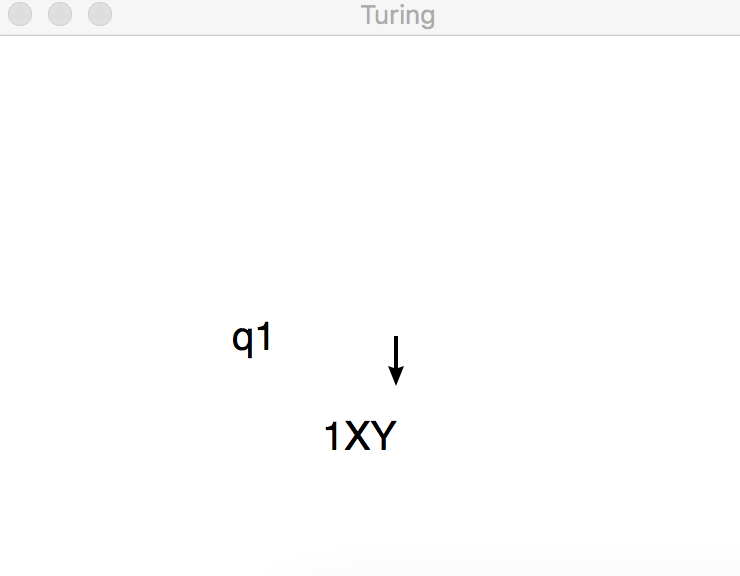
\includegraphics[scale=.6]{img/prueba3.png}
			\caption{Resultados prueba (3)}
			\label{fig:maquin4}
		\end{center}
	\end{figure}
	\begin{figure}[H]
		\begin{center}
			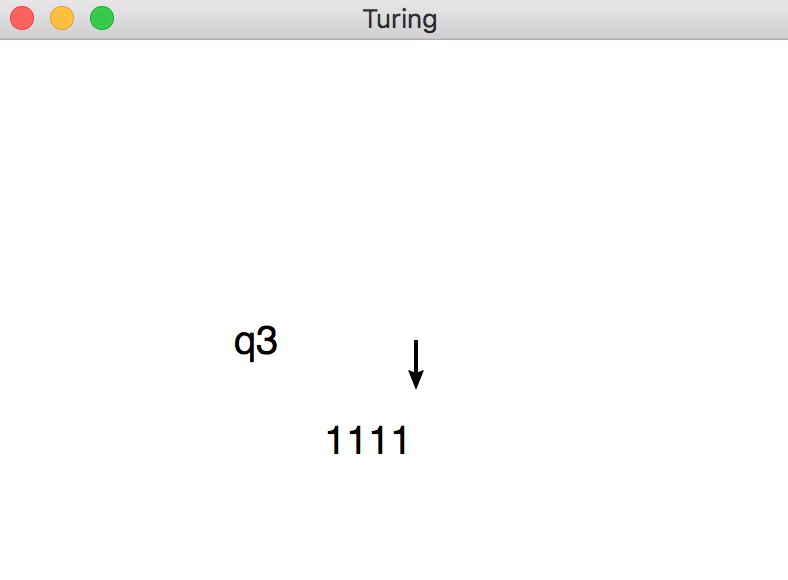
\includegraphics[scale=.6]{img/prueba4.png}
			\caption{Resultados prueba (4)}
			\label{fig:maquina5}
		\end{center}
	\end{figure}